% -----------------------------------------------------------------------------
% The MIT License (MIT)
%
% Copyright (c) 2015 Pejman Ghorbanzade
%
% Permission is hereby granted, free of charge, to any person obtaining a copy
% of this software and associated documentation files (the "Software"), to deal
% in the Software without restriction, including without limitation the rights
% to use, copy, modify, merge, publish, distribute, sublicense, and/or sell
% copies of the Software, and to permit persons to whom the Software is
% furnished to do so, subject to the following conditions:
%
% The above copyright notice and this permission notice shall be included in
% all copies or substantial portions of the Software.
%
% THE SOFTWARE IS PROVIDED "AS IS", WITHOUT WARRANTY OF ANY KIND, EXPRESS OR
% IMPLIED, INCLUDING BUT NOT LIMITED TO THE WARRANTIES OF MERCHANTABILITY,
% FITNESS FOR A PARTICULAR PURPOSE AND NONINFRINGEMENT. IN NO EVENT SHALL THE
% AUTHORS OR COPYRIGHT HOLDERS BE LIABLE FOR ANY CLAIM, DAMAGES OR OTHER
% LIABILITY, WHETHER IN AN ACTION OF CONTRACT, TORT OR OTHERWISE, ARISING FROM,
% OUT OF OR IN CONNECTION WITH THE SOFTWARE OR THE USE OR OTHER DEALINGS IN
% THE SOFTWARE.
% -----------------------------------------------------------------------------

\def \topDirectory {../..}

\documentclass[10pt, compress]{beamer}

\usepackage{\topDirectory/template/style/directives}
%%%%%%%%%%%%%%%%%%%%%%%%%%%%%%%%%%%%%%%%%%%%%%%%%%%%%%%%%%%%%%%%%%%%%%%%%%%%%%
% CS110: Introduction to Computing
% Copyright 2015 Pejman Ghorbanzade <mail@ghorbanzade.com>
% Creative Commons Attribution-ShareAlike 4.0 International License
% https://github.com/ghorbanzade/UMB-CS110-2015S/blob/master/LICENSE
%%%%%%%%%%%%%%%%%%%%%%%%%%%%%%%%%%%%%%%%%%%%%%%%%%%%%%%%%%%%%%%%%%%%%%%%%%%%%%

\course{id}{CS110}
\course{name}{Introduction to Computing}
\course{venue}{Tue/Thu, 5:30 PM - 6:45 PM}
\course{semester}{Spring 2015}
\course{department}{Department of Computer Science}
\course{university}{University of Massachusetts Boston}

\instructor{name}{Pejman Ghorbanzade}
\instructor{title}{}
\instructor{position}{Student Instructor}
\instructor{email}{pejman@cs.umb.edu}
\instructor{phone}{617-287-6419}
\instructor{office}{S-3-124B}
\instructor{office-hours}{Tue/Thu 19:00-20:30}
\instructor{address}{University of Massachusetts Boston, 100 Morrissey Blvd., Boston, MA}

\usepackage{\topDirectory/template/style/beamerthemeUmassLecture}
\doc{number}{14}
%\setbeamertemplate{footline}[text line]{}

\begin{document}
\prepareCover

\section{Course Administration}

\begin{frame}[fragile]
\frametitle{Course Administration}
Assignment 5 released. Due on April 30, 2015 at 17:30 PM.
\end{frame}

\begin{frame}[fragile]
	\frametitle{Overview}
	\begin{itemize}
		\item[] Polymorphism
		\begin{itemize}
			\item[] Introduction
			\item[] Method Overloading
			\item[] Method Overriding
			\item[] Subtyping
		\end{itemize}
	\end{itemize}
\end{frame}

\plain{}{Polymorphism}

\section{Introduction}

\begin{frame}[fragile]
	\frametitle{Polymorphism}
	\begin{figure}\centering
		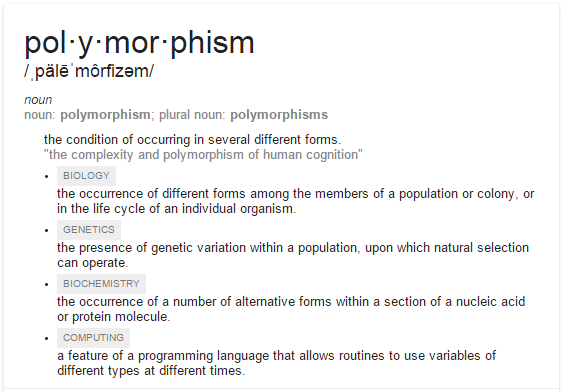
\includegraphics[width=\textwidth]{\topDirectory/template/images/polymorphism.png}
	\end{figure}
\end{frame}

\begin{frame}[fragile]
	\frametitle{Polymorphism}
	\begin{block}{Polymorephism in Computer Science}
		\begin{itemize}
			\item[] \textbf{Ad-hoc Polymorphism} A function denotes different and potentially heterogeneous implementations depending on a limited range of individually specified types and combinations
			\item[] \textbf{Parametric Polymorphism} A function developed without mention of any specific type and thus can be used transparently with any number of new types
			\item[] \textbf{Inclusion Polymorphism} A concept wherein a name may denote instances of many different classes as long as they are related by some common superclass
		\end{itemize}
	\end{block}
\end{frame}

\begin{frame}[fragile]
	\frametitle{Polymorphism}
	\begin{block}{(Ad-hoc) Polymorephism in Java}
		\begin{itemize}
			\item[] \textbf{Compile-Time Polymorphism} allows development of methods with the same name but with different parameter list
			\item[] \textbf{Run-Time Polymorphism} allows unique implementation of methods of the super class in sub classes
		\end{itemize}
	\end{block}
	\begin{block}{(Inclusion) Polymorphism in Java}
		\begin{itemize}
			\item[] \textbf{Subtyping} allows the subclass object to be referenced via the super class.
		\end{itemize}
	\end{block}
\end{frame}

\begin{frame}[fragile]
	\frametitle{Polymorphism}
	\begin{block}{Advantage}
		\begin{itemize}
			\item[] \textbf{Compile-Time Polymorphism} enables \alert{method overloading} where multiple methods of same name but different parameter list can be developed in a class.
			\item[] \textbf{Run-Time Polymorphism} enables \alert{method overriding} where a method previously implemented in The super class can be overridden in the subclass.
			\item[] \textbf{Subtyping} allows instantiation of an object during compile-time while determining its type in run-time.
		\end{itemize}
	\end{block}
\end{frame}

\section{Method Overloading}

\begin{frame}[fragile]
	\frametitle{Polymorphism}
	\begin{block}{Objective}
		Write a program \texttt{BigOcean.java} that controls movement of a fish in a vast ocean.
	\end{block}
\end{frame}

\begin{frame}[fragile]
	\frametitle{Polymorphism}
	\begin{block}{Class \texttt{Fish.java} (Page 1)}
		\begin{minted}[fontsize=\small,tabsize=8, linenos, firstnumber=1]{java}
public class Fish {
	// attributes
	private double posX;
	private double posY;
	// constructors
	public Fish() {
		posX = 0;
		posY = 0;
	}
	// print position
	public void showPosition() {
		System.out.printf("moved to [%.1f, %.1f]\n",
				this.posX, this.posY);
	}
		\end{minted}
	\end{block}
\end{frame}

\begin{frame}[fragile]
	\frametitle{Polymorphism}
	\begin{block}{Class \texttt{Fish.java} (Page 2)}
		\begin{minted}[fontsize=\small,tabsize=8, linenos, firstnumber=15]{java}
	// fish moves some random distance in some random direction
	public void move() {
		double direction = 2 * Math.PI * Math.random();
		double distance = 10 * Math.random();
		this.posX += distance * Math.cos(direction);
		this.posY += distance * Math.sin(direction);
	}
	// fish moves [distance] meters in some random direction
	public void move(double distance) {
		double direction = 2 * Math.PI * Math.random();
		this.posX += distance * Math.cos(direction);
		this.posY += distance * Math.sin(direction);
	}
		\end{minted}
	\end{block}
\end{frame}

\begin{frame}[fragile]
	\frametitle{Polymorphism}
	\begin{block}{Class \texttt{Fish.java} (Page 3)}
		\begin{minted}[fontsize=\small,tabsize=8, linenos, firstnumber=28]{java}
	// fish moves to [posX, posY]
	public void move(double posX, double posY) {
		this.posX = posX;
		this.posY = posY;
	}
	// fish moves [distance] meters toward [someFish]
	public void move(double distance, Fish someFish) {
		double direction = Math.atan2(
				someFish.getPosY() - this.posY,
				someFish.getPosX() - this.posX
				);
		this.posX += distance * Math.cos(direction);
		this.posY += distance * Math.sin(direction);
	}
		\end{minted}
	\end{block}
\end{frame}

\begin{frame}[fragile]
	\frametitle{Polymorphism}
	\begin{block}{Class \texttt{Fish.java} (Page 4)}
		\begin{minted}[fontsize=\small,tabsize=8, linenos, firstnumber=42]{java}
	// getters and setters
	public double getPosX() {
		return posX;
	}
	public double getPosY() {
		return posY;
	}
}
		\end{minted}
	\end{block}
\end{frame}

\begin{frame}[fragile]
	\frametitle{Polymorphism}
	\begin{block}{Class \texttt{BigOcean.java}}
		\begin{minted}[fontsize=\small,tabsize=8, linenos, firstnumber=1]{java}
public class BigOcean {
	public static void main(String[] args) {
		Fish fish1 = new Fish();
		fish1.move(10);
		fish1.showPosition();
		fish1.move();
		fish1.showPosition();
		fish1.move(10, 10);
		fish1.showPosition();
		Fish fish2 = new Fish();
		fish2.move(5, fish1);
		fish2.showPosition();
	}
}
		\end{minted}
	\end{block}
\end{frame}

\section{Method Overriding}

\begin{frame}[fragile]
	\frametitle{Polymorphism}
	\begin{block}{Objective}
		Write a program \texttt{BigOcean2.java} that using the previously developed class \texttt{Fish.java} controls movement of a salmon in a vast ocean.
	\end{block}
\end{frame}

\begin{frame}[fragile]
	\frametitle{Polymorphism}
	\begin{block}{Class \texttt{Salmon.java}}
		\begin{minted}[fontsize=\small,tabsize=8, linenos, firstnumber=1]{java}
public class Salmon extends Fish {
	@Override
	public void move() {
		super.move();
		System.out.println("The salmon just moved!");
	}
	public void sing() {
		System.out.println("Let it go!");
	}
}
		\end{minted}
	\end{block}
\end{frame}

\begin{frame}[fragile]
	\frametitle{Polymorphism}
	\begin{block}{Class \texttt{BigOcean2.java}}
		\begin{minted}[fontsize=\small,tabsize=8, linenos, firstnumber=1]{java}
public class BigOcean2 {
	public static void main(String[] args) {
		Salmon fish1 = new Salmon();
		fish1.move();
		fish1.showPosition();
		fish1.sing();
	}
}
		\end{minted}
	\end{block}
	\begin{block}{Output}
		\begin{verbatim}
		The salmon just moved!
		moved to [0.8, 1.3]
		Let it go!
		\end{verbatim}
	\end{block}
\end{frame}

\section{Subtyping}

\begin{frame}[fragile]
	\frametitle{Polymorphism}
	\begin{block}{Class \texttt{BigOcean3.java}}
		\begin{minted}[fontsize=\small,tabsize=8, linenos, firstnumber=1]{java}
public class BigOcean3 {
	public static void main(String[] args) {
		Salmon fish1 = new Salmon();
		Fish fish2 = fish1;
		Object fish3 = fish2;
		System.out.println(fish3.equals(fish1)); // prints true
	}
}
		\end{minted}
	\texttt{fish1}, \texttt{fish2} and \texttt{fish3} all refer to the same Salmon.
	\end{block}
\end{frame}

\begin{frame}[fragile]
	\frametitle{Polymorphism}
	\begin{block}{Class \texttt{BigOcean3.java}}
		\begin{minted}[fontsize=\small,tabsize=8, linenos, firstnumber=1]{java}
public class BigOcean3 {
	public static void main(String[] args) {
		Salmon fish1 = new Salmon();
		Fish fish2 = fish1;
		fish1.sing();
		fish2.sing();
	}
}
		\end{minted}
	\end{block}
\end{frame}

\begin{frame}[fragile]
	\frametitle{Polymorphism}
	\begin{block}{Output}
\begin{verbatim}	Let it go!
	The method sing() is undefined for the type Fish
\end{verbatim}
	\end{block}
	\begin{block}{Problem Statement}
		Compiler treats \texttt{fish2} like any other instance of class Fish.
	\end{block}
	\begin{block}{Lesson Learned}
		Subtyping affects how compiler identifies the objects.
	\end{block}
\end{frame}

\begin{frame}[fragile]
	\frametitle{Polymorphism}
	\begin{block}{Class \texttt{BigOcean3.java}}
		\begin{minted}[fontsize=\small,tabsize=8, linenos, firstnumber=1]{java}
public class BigOcean3 {
	public static void main(String[] args) {
		Salmon fish1 = new Salmon();
		Fish fish2 = new Salmon();
		fish1.move();
		fish2.move();
	}
}
		\end{minted}
	\end{block}
\end{frame}

\begin{frame}[fragile]
	\frametitle{Polymorphism}
	\begin{block}{Output}
\begin{verbatim}	The salmon just moved!
	The salmon just moved!
\end{verbatim}
	\end{block}
	\begin{block}{Justification}
		Program passes compilation because compiler finds a method \texttt{move()} in class \texttt{Fish} for \texttt{fish2}. In run-time however, method \texttt{move()} of class \texttt{Salmon} is invoked.
	\end{block}
	\begin{block}{Lesson Learned}
		Subtyping does not affect how JVM identifies objects.
	\end{block}
\end{frame}

\begin{frame}[fragile]
	\frametitle{Polymorphism}
	\begin{block}{Notes}
		\begin{itemize}
			\item[] Any object with more than one IS-A relation is polymorphic
			\item[] Any object is an instance of class \texttt{Object}, thus polymorphic
		\end{itemize}
	\end{block}
\end{frame}

\plain{}{Keep Calm\\and\\Think Object-Oriented}

\end{document}
